% debut d'un fichier latex standard
\documentclass[a4paper,12pt,twoside]{article}
% Tout ce qui suit le symbole "%" est un commentaire
% Le symbole "\" désigne une commande LaTeX

% pour l'inclusion de figures en eps,pdf,jpg, png
\usepackage{graphicx}

% quelques symboles mathematiques en plus
\usepackage{amsmath}

% le tout en langue francaise
\usepackage[french]{babel}

% on peut ecrire directement les caracteres avec l'accent
%    a utiliser sur Linux/Windows (! dépend de votre éditeur !)
\usepackage[utf8]{inputenc}
\usepackage[T1]{fontenc}

%    a utiliser sur le Mac ???
%\usepackage[applemac]{inputenc}

% pour l'inclusion de liens dans le document
\usepackage[colorlinks,bookmarks=false,linkcolor=blue,urlcolor=blue]{hyperref}

\paperheight=297mm
\paperwidth=210mm

\setlength{\textheight}{235mm}
\setlength{\topmargin}{-1.2cm} % pour centrer la page verticalement
%\setlength{\footskip}{5mm}
\setlength{\textwidth}{15.5cm}
\setlength{\oddsidemargin}{0.5cm}
\setlength{\evensidemargin}{0.5cm}

\pagestyle{plain}

% nouvelles commandes LaTeX, utilis\'ees comme abreviations utiles
\def \be {\begin{equation}}
\def \ee {\end{equation}}
\def \dd  {{\rm d}}

\newcommand{\mail}[1]{{\href{mailto:#1}{#1}}}
\newcommand{\ftplink}[1]{{\href{ftp://#1}{#1}}}
%
% latex SqueletteRapport.tex      % compile la source LaTeX
% xdvi SqueletteRapport.dvi &     % visualise le resultat
% dvips -t a4 -o SqueletteRapport.ps SqueletteRapport % produit un PostScript
% ps2pdf SqueletteRapport.ps      % convertit en pdf

% pdflatex SqueletteRapport.pdf    % compile et produit un pdf

% ======= Le document commence ici ======

\begin{document}

% Le titre, l'auteur et la date
\title{Squelette d'un rapport en \LaTeX, version 1.1}
\author{$\nabla$Un Nom, Autre Nom\\  % \\ pour fin de ligne
{\small \mail{un.nom@epfl.ch},\mail{autre.nom@epfl.ch}}}
\date{\today}\maketitle
\tableofcontents % Table des matieres
\[ \int \oint f=m\overrightarrow{a} \]
% Quelques options pour les espacements entre lignes, l'indentation
% des nouveaux paragraphes, et l'espacement entre paragraphes
\baselineskip=16pt
\parindent=0pt
\parskip=12pt

\section{Préambule}

Un document \LaTeX{} de type article  est subdivis\'e en sections, sous-sections, sous-sous sections.                                   L'utilisateur n'a pas
besoin de se pr\'eoccupper
de la

 num\'erotation, ni de la police utilis\'ee, ni des espacements.
%\end{document}

\section{Introduction} %------------------------------------------

Bonjour!

\LaTeX{} est un syst\`eme de pr\'eparation de documents de qualit\'e, utilis\'e sp\'ecialement dans les domaines scientifiques et techniques. \LaTeX{} n'est \textbf{pas} un logiciel de traitement de texte.Au contraire, \LaTeX{} incite les auteurs \`a ne \textit{pas} se soucier eux-m\^emes de l'apparence de leurs documents et leur permet de se concentrer sur leur contenu.

\section{Nouvelle section}

\LaTeX{} fonctionne comme un langage de programmation, dans ce sens que le fichier \textit{source} (ici SqueletteRapport.tex), doit \^etre compil\'e avant de produire un r\'esultat. A la ligne de commande Linux, tapez:
\begin{verbatim}
 latex SqueletteRapport.tex
\end{verbatim}
puis:
\begin{verbatim}
 xdvi SqueletteRapport.dvi &
\end{verbatim}
pour pr\'evisualiser le r\'esultat. Ensuite, on produit un fichier PostScript avec la commande
\begin{verbatim}
dvips -t a4 -o SqueletteRapport.ps SqueletteRapport
\end{verbatim}
que l'on convertit en pdf avec
\begin{verbatim}
ps2pdf SqueletteRapport.ps
\end{verbatim}
Cette derni\`ere commande produira un fichier \verb+SqueletteRapport.pdf+.

Au lieu de la combinaison des commandes \verb+latex+, \verb+dvips+ et \verb+ps2pdf+, on peut utiliser la commande:
\begin{verbatim}
pdflatex SqueletteRapport.tex
\end{verbatim}
qui d'un coup compile et produit un \verb+.pdf+.

Voir en section\ref{SABC} la remarque concernant le format des fichiers graphiques pour leur inclusion comme figures dans le document.

Mentionnohkjhns qu'il existe dess logiciels comme \verb+TeXworks+ (freeware) qui int\`grent un \'editeur, un interface graphique utilisateur et un pr\'evisualisateur de pdf.

Il y a plusieurs ressources sur le kjhe site Moodle du cours dans le r\'epertoire \verb+Ressources LaTeX+. En particulier, la "feuille de triche" \verb+latexsheet.pdf+ qui r\'esume, sur une feuille, les commandes \LaTeX{} les plus couramment utilis\'ees. La liste compl\`ete des symboles sp\'eciaux et la description des commandes \LaTeX{} qui les produisent se trouvent dans \verb+symbols-a4.pdf+.

En guise  d'introduction, on introduira quelques commandes \LaTeX{}.
Et on corrigera les fautes d'orthograffe.
Les espaces        et        les         fins                       de    lignes
dans
le
fichier \LaTeX{} sont        ignor\'es. Une ligne vide dans le fichier source veut dire qu'un nouveau paragraphe commence dessous.










Mettre plusieurs lignes vides n'a pas plus d'effet qu'en mettre une seule.



Les accen khew kjhts grave (g\`ele), aig\"u (d\'ebut), circonflexe (b\^ete), tr\'ema
sur le i : (na\"\i ve), et la c\'edille s'\'ecrivent comme \c{c}a:
\begin{verbatim}
Les accents grave (g\`ele),
aig\"u (d\'ebut), circonflexe (b\^ete),
tr\'ema sur le i : (na\"\i ve), et la c\'edille s'\'ecrivent comme
\c{c}a
\end{verbatim}

On a plac\'e les lignes ci-dessus entre \verb|\begin{verbatim}| et
\verb|\end{verbatim}| pour qu'elles apparaissent exactement comme elles
sont dans le fichier source. Pour faire de m\^eme dans un paragraphe,
on place le texte entre \verb|\verb|$|$ et  $|$.

Comme le symbole \verb|%| signale que tout ce qui suit est un commentaire et sera donc ignor\'e, il faut, pour \'ecrire \%, le pr\'ec\'eder du symbole \verb|\|, ou comme \verb+\verb|\|+.
Ainsi le symbole \% sera visible, avec ce qui suit!

Lorsqu'on veut inscrire les accents directement avec un éditeur, il faut faire attention de
choisir l'encodage UTF-8. Par exemple avec kile, aller sous Settings -> Configure -> Kile -> (panneau de gauche) Editor -> Open/Save, puis sous l'onglet General, s\'electionner Encoding: Unicode (UTF-8). Sauver, puis quitter et rouvrir kile. Ensuite, taper les caractères avec accent.

Les \'equations sont soit des expressions ins\'er\'ees dans un paragraphe, par exemple
$F=ma$, \(E=mc^2\) ou \begin{math} p=mv \end{math},
plac\'ees entre \$ et \$ ou entre \verb|\begin{math}| et \verb|\end{math}|,
soit occupent une ligne s\'epar\'ee, entre \verb|\[| et \verb|\]|,
\[ E=mc^2, \]
ou, avec num\'erotation {\it automatique}, entre \verb|\begin{equation}|
et \verb|\end{equation}|:
\begin{equation}
y_{n+1}=y_n+f(y_{njk},t_n)\Delta t g^{\alpha+2}
\end{equation}
\begin{equation}
E=mc^2
\end{equation}
\begin{equation}
\frac{d^2y}{dt^2} = f(y,t)
\end{equation}
Comme on \'ecrira souvent des \'equations, il peut \^etre int\'eressant de d\'efinir de nouvelles commandes. Cela se fait dans le pr\'eambule, c.a.d. avant \verb|\begin{document}|, par exemple:
\begin{verbatim}
\def \be {\begin{equation}}
\def \ee {\end{equation}}
\def \dd  {{\rm d}}
\end{verbatim}
Ainsi la l'\'ecriture s'en trouvera simplifi\'ee:
\be
\frac{\dd y}{\dd t} =    f(y,t)      . % Commentaire: en mode \'equation, les espaces du fichier source sont ignor\'es.
\ee

On rajoute des ``d\'ecorations'' sur les symboles, par exemple pour un vecteur
$\vec{F}=m\vec{a}$, ou $\vec{AB}=\vec{OB}-\vec{OA}$, ou
$\overrightarrow{AB}$.  %Voir p.33 des transparents.

\subsection{R\'ef\'erences crois\'ees} \label{sec:figures} %---------------

\LaTeX{} a un syst\`eme de r\'ef\'rences crois\'ees pour plusieurs choses.
Par exemple pour les \'equations. On place \verb|\label{NOMDULABEL}| entre
\verb|\begin{equation}| et \verb|\end{equation}|.   Soit

\begin{equation} \label{NOMDULABEL}
\vec{F} =m\vec{a}
\end{equation}

\begin{eqnarray}
F &=& ma  \nonumber\\
&+& mc^2
\end{eqnarray}

On fait r\'ef\'erence \`a cette \'equation avec la commande \verb|\ref{NOMDULABEL}|: de l'Eq.(\ref{NOMDULABEL}), on en tire $F_x=mx''$.

On fait r\'ef\'erence \`a la sous-section \ref{SABC} avec la commande
\verb|\ref{SABC}|.

% Voici une figure 'flottante', c'est a dire que c'est Latex qui va vous placer
% la figure la ou il lui semble bon.
\begin{figure} %------------------------------------------------
% si on utilise latex, les fichiers graphiques doivent etre au format .eps
% si on utilise pdflatex, ils doivent etre au format pdf, png ou jpg
%\centerline{\includegraphics[width=0.9\linewidth,angle=0]{Plot}}
% ou
\begin{center}
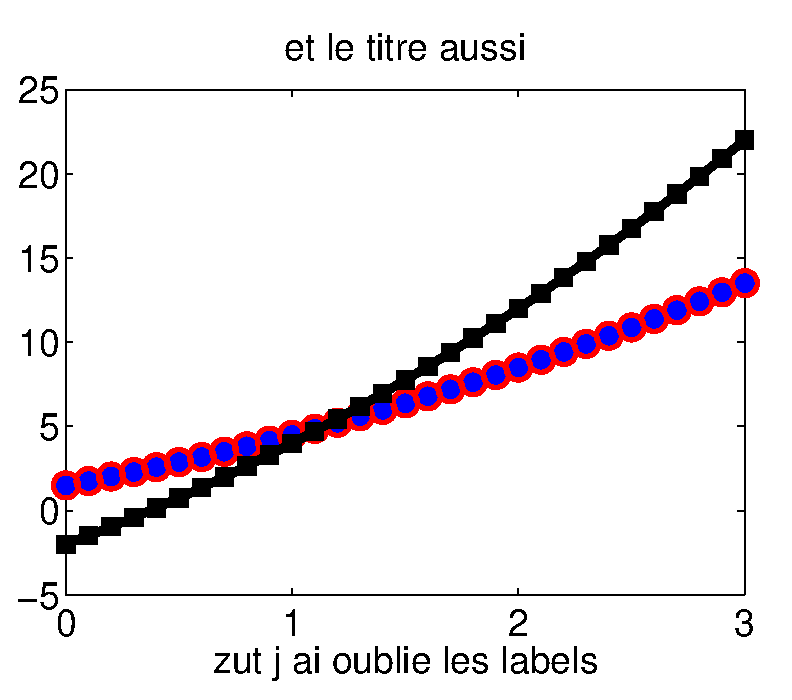
\includegraphics[width=7cm,angle=0]{ohmabellefigure}
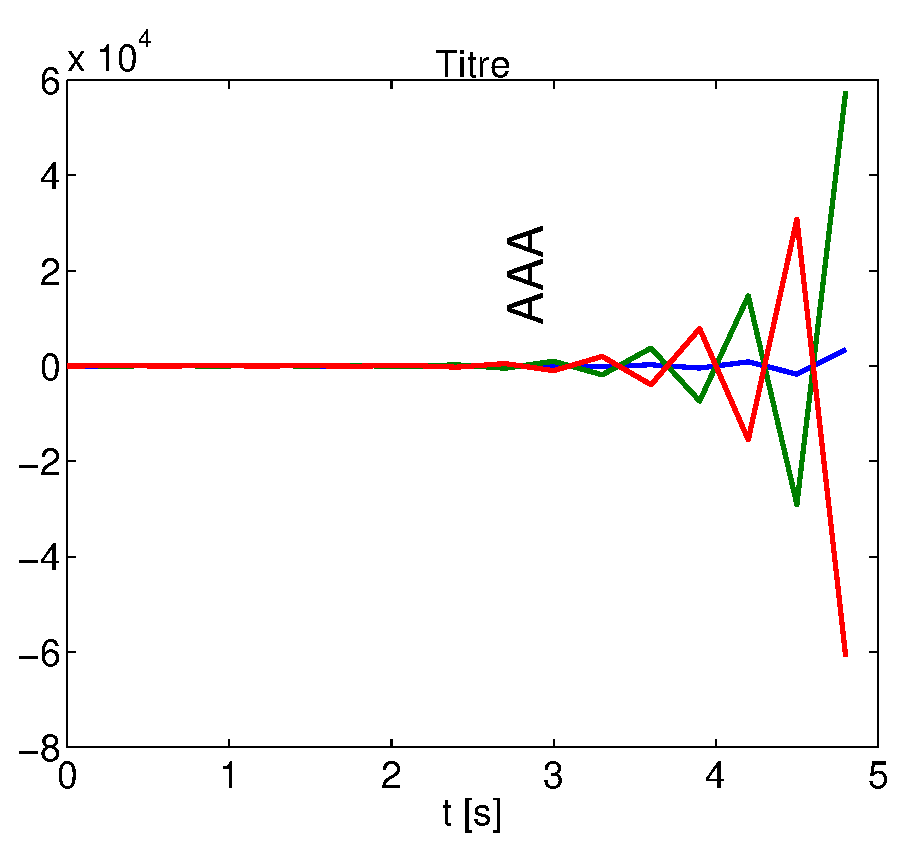
\includegraphics[width=7cm,angle=0]{aa}
\end{center}
% la legende est dans \caption{...}
\caption{\em \label{fig:Plot}
Ceci est une l\'egende.
}
\end{figure} %---------------------------------------------------

On fait r\'ef\'erence \`a la FIG.\ref{fig:Plot} avec la commande
\verb|\ref{fig:Plot}|.

Les r\'ef\'erences bibliographiques \cite{Duschmoll_PRL}
s'obtiennent avec \verb|\cite{Duschmoll_PRL}|
ou avec \cite{Abi_Science} \verb|\cite{Abi_Science}|.

\subsection{Inclure des figures dans le document} \label{SABC}
%--------------------------------------
Remarque: On a plac\'e un label dans cette sous-section: \verb|\label{SABC}|.

Si on compile la source \LaTeX{} avec la commande
\verb|latex SqueletteRapport.tex|,
les figures doivent \^etre au format \verb|eps|.

Si on compile avec la commande
\verb|pdflatex SqueletteRapport.tex|,
les figures doivent \^etre au format \verb|pdf| ou \verb|png|
ou \verb|jpeg|.

On inclut les figures dans le document dans l'environnement \verb|figure|, entre \verb|\begin{figure}| et \verb|\end{figure}|, avec la commande

\verb|\includegraphics[width=...cm, ...]{nom_du_fichier} |

Il est mieux de ne PAS mettre explicitement l'extension (.eps ou .pdf ou .png ou .jpg) après le nom du fichier à inclure. latex cherchera aa.eps, pdflatex cherchera aa.pdf ou  aa.png ou aa.jpg

%-----------------------------------------------------------
\section{La structure en sections}

\subsection{et en sous-sections}

\subsubsection{et en sous-sous-sections}

%\subsubsubsection{et en sous-sous-sous-sections}

%-----------------------------------------------------------
\section{Conclusions}

%-----------------------------------------------------------


\begin{thebibliography}{99}
\bibitem{Duschmoll_PRL}
 A. Duschmoll, R. Schnok, {\it Phys. Rev. Lett.} {\bf 112} 010015 (2010)
\bibitem{Abi_Science}
 D.D. Abi, {\it et al}, {\it Science} {\bf 22} 1242 (2007)
\end{thebibliography}

\end{document} %%%% THE END %%%%
